\documentclass[autodetect-engine,dvipdfmx,platex]{deimj}
\usepackage{latexsym}
\usepackage{booktabs}
\usepackage{color}
\usepackage{colortbl}
\usepackage{graphicx}
\usepackage{amsmath}
\usepackage{bm}
\usepackage{cite}
\usepackage{multirow}
\usepackage[hidelinks]{hyperref}
\usepackage{pxjahyper}
%\usepackage[switch]{lineno}
\usepackage{caption}
\usepackage{subcaption}
\usepackage[section]{placeins}
\usepackage{float}

% 印刷位置調整 %
% 必要に応じて値を変更してください．
\hoffset -10mm % <-- 左に 10mm 移動
\voffset -10mm % <-- 上に 10mm 移動

\newcommand{\AmSLaTeX}{%
 $\mathcal A$\lower.4ex\hbox{$\!\mathcal M\!$}$\mathcal S$-\LaTeX}
\newcommand{\PS}{{\scshape Post\-Script}}
\def\BibTeX{{\rmfamily B\kern-.05em{\scshape i\kern-.025em b}\kern-.08em
 T\kern-.1667em\lower.7ex\hbox{E}\kern-.125em X}}

\papernumber{DEIM Forum 2026 XX-Y}

\jtitle{行動分布の不確実性を考慮した方策再利用型転移学習}
\authorlist{%
 \authorentry[c5625291@aoyama.jp]{塚原 悠生}{Yusei Tsukahara}{ShizuokaUniv}%
 \authorentry[saitoh@ise.aoyama.ac.jp]{齊藤 史哲}{Humiaki Saitou}{ShizuokaUniv}%
}
\affiliate[ShizuokaUniv]{青山学院大学大学院理工学研究科\hskip1zw
  〒252--5258 神奈川県相模原市中央区淵野辺本町5-10-1}
 {Faculty of Informatics, Shizuoka University\\
  3--5--1, Johoku, Naka-ku, Hamamatsu, Shizuoka,432--8011, Japan}

\begin{document}
%\linenumbers %このオプションは投稿時には無効にすること
\pagestyle{empty}

%%%%%%%%%%%%%%%%%%%%%%%%%%%%
% アブストラクト（300字程度）
%%%%%%%%%%%%%%%%%%%%%%%%%%%%
\begin{jabstract}
近年，強化学習の実運用では環境変化に対し
短時間で性能を回復する適応性が求められる．
本研究では，方策再利用（Policy Reuse）
におけるエピソードごとの方策選択を多腕バンディットとして捉え，
従来のBoltzmann選択に加えてε-greedyとUCBを導入し，
格子状迷路で比較した．さらに，ゴール到達報酬のみと，
ステップ負報酬＋壁衝突ペナルティの2種の報酬設計で影響を検証した．
実験の結果，いずれの報酬設計でもPRQ系列は通常のQ学習を一貫して
上回り学習効率が向上した一方，最良の選択手法はタスクや
報酬構造に依存して変化することを示した．
以上より，方策選択の設計が再利用効果と安定性を左右することが示唆された．

\end{jabstract}

%%%%%%%%%%%%%%%%%%%%%%%%%%%%
% キーワード
%%%%%%%%%%%%%%%%%%%%%%%%%%%%
\begin{jkeyword}
強化学習，転移学習，迷路探索タスク，バンディットアルゴリズム
\vspace{2em}
\end{jkeyword}


%%%%%%%%%%%%%%%%%%%%%%%%%%%%
% 本文
%%%%%%%%%%%%%%%%%%%%%%%%%%%%
\maketitle

% 0章：LateXの使い方
%\input{../contents/text/latex}

% 1章：はじめに
\section{はじめに}
近年，強化学習を実運用へ適用するためには，環境が変化しても短時間で性能を回復・向上できる適応性が重要である．
強化学習は，エージェントが試行錯誤を通じて最適な行動方策を獲得する枠組みであり
\cite{SuttonBarto1998,WatkinsDayan1992}，
ゲームやロボティクスに加え，物流・製造計画など多様な領域での活用が期待されている．
一方で，反復的な探索と学習には多大な試行回数と計算時間を要し，
実環境では学習効率の低さが主要な課題となる
\cite{Thrun1995}．
例えば倉庫の入出庫スケジュール最適化や工場のジョブショップスケジューリングでは，
設備配置や需要が変化するたびにゼロから学習し直すことは現実的でない場合が多い．

この課題に対する有力なアプローチとして転移学習がある
\cite{TaylorWhitesonStone2007}．
転移学習では，変化前の環境（ソース）で獲得した知識を新しい環境（ターゲット）の学習に再利用することで，
学習初期の性能向上や総学習時間の短縮が期待できる．
とりわけ，方策や価値関数の再利用は環境構造が類似する場合に効果的であるが，
ソース知識をどの程度信頼して利用するかは容易ではなく，
不適切な再利用はターゲット適応を阻害しうる
\cite{TaylorKuhlmannStone2008}．

過去に学習した方策を探索へ組み込む枠組みとして，Fern\'andez と Veloso は
方策ライブラリからエピソード単位で方策を選択し，確率的に再利用する手法を提案している
\cite{Fernandez2006}．
また，学習を改善するために追加知識を探索へ注入する研究として，
助言ルールによる学習支援
\cite{MaclinShavlik1996}，
模倣に基づく方策獲得
\cite{NicolescuMataric2003}，
階層化による知識再利用
\cite{BartoMahadevan2003,KonidarisBarto2007}
などが報告されている．

本研究では，転移学習の枠組みにおける方策選択手法の影響を体系的に評価することを目的とする．
具体的には，既存研究で用いられているボルツマン選択に加え，
$\varepsilon$-greedy および UCB を導入し，
3種類のバンディットアルゴリズムに基づく方策選択を同一条件下で比較実験する．
さらに，報酬設計の違いが比較結果に与える影響にも着目し，
従来の報酬に加えて，各ステップでのマイナス報酬および壁衝突時のペナルティを導入した報酬設計においても同様の検証を行う．
これにより，探索と活用のバランスが異なる方策選択が，
報酬構造の変化に対してどのように挙動を変えるのかを明らかにし，
実運用を見据えた転移強化学習の設計指針を得ることを目指す．



% 2章：関連研究
\section{関連研究}
転移強化学習では，ソース環境で得た知識をターゲット環境へ
再利用することで学習効率を改善する試みが広く研究されている．
なかでも過去に学習した方策を学習中の探索に組み込む「方策再利用」は，
環境構造が類似する場合に学習初期の性能を押し上げる一方，
不適切な再利用は負の転移を招くため，再利用の制御が重要となる．

Fern\'andez と Veloso は，
複数の過去方策を保持した方策ライブラリから，
ターゲット環境における学習を支援するために
過去方策を確率的に再利用する枠組みを提案した 
\cite{Fernandez2006}．
方策ライブラリ $\mathcal{L}=\{\Pi_1,\Pi_2,\ldots,\Pi_n\}$ 
と学習中の新方策 $\Pi_{\Omega}$ を候補とし，
エピソードごとに1つの方策を選択して実行する．
各方策 $\Pi_i$ には有効性指標 $W_i$（Reuse Gain）を保持し，
得られたリターンに基づいて更新する．
文献\cite{Fernandez2006}では，最大の $W$ を持つ方策指標として
\begin{equation}
j^\ast = \arg\max_{i=1,\ldots,n} W_i
\tag{3}
\end{equation}
を定義し，候補方策 $\Pi_j$ の選択確率を
\begin{equation}
P(\Pi_j)=\frac{\exp(\tau W_j)}{\sum_{p=0}^{n}\exp(\tau W_p)}
\tag{4}
\end{equation}
で与える（$p=0$ は新方策に対応）．

また，同研究では，選択した方策に常に従うのではなく，
再利用率 $\psi$ により探索を混合する実行戦略（$\pi$-reuse）を導入している．
具体的には，時刻 $t$ の状態 $s_t$ における行動 $a_t$ を
\begin{equation}
a_t =
\begin{cases}
\displaystyle \arg\max_{a} Q_{\Pi_j}(s_t,a)
& (\text{w/ prob. } \psi)\\[3pt]
\displaystyle \arg\max_{a} Q_{\Pi_{\mathrm{new}}}(s_t,a)
& (\text{w/ prob. } 1-\psi)
\end{cases}
\tag{5}
\end{equation}

のように決定し，
過去方策の過信を抑えつつターゲット環境での学習を進める．

以上を踏まえ，本研究はPRQ-Learningの枠組みを保ったまま
方策ライブラリからの方策選択部を拡張し，
ボルツマン選択に限定しない比較を行う点に特徴がある．


% 3章：提案事項
\section{提案手法}
本研究では，方策再利用（Policy Reuse）の枠組みにおける
「エピソードごとに採用する方策の選択」を多腕バンディット
として捉え，
既存研究で用いられるボルツマン選択に加えて 
$\varepsilon$-greedy および UCB を適用し，
その性能差を比較する．
さらに，報酬設計を2種類用意し，
報酬構造の違いが各手法の優劣に与える影響も検証する．

\subsection{方策再利用の枠組み}
ソース側で学習した方策の集合（Policy Library）を
\begin{equation}
\mathcal{L}=\{\pi_1,\pi_2,\dots,\pi_K\}
\end{equation}
とし，ターゲットで学習中の方策を $\pi_{\mathrm{new}}$ とする．
各エピソード開始時に $\mathcal{L}\cup\{\pi_{\mathrm{new}}\}$ 
から1つの方策を選択し，
エピソード中は選択方策を参照して行動を決定する．
エピソード終了後，得られたリターンに基づき各方策の推定価値
 $V_i$ を更新し，次エピソードの方策選択に用いる．

また，エピソード内の行動決定は再利用率 $\psi$ により統一し，
確率 $\psi$ で選択方策の推奨行動を採用し，
確率 $1-\psi$ で探索行動を採用する．
これにより，本研究では方策選択アルゴリズムの差に着目した
比較を行う．

\subsection{方策選択アルゴリズム（3手法）}
各方策 $\pi_i$ について推定価値 $V_i$ と選択回数 $N_i$ を保持し，
エピソードごとに以下のいずれかで方策を選択する．

\paragraph{ボルツマン選択（Softmax）}
\begin{equation}
P(\pi_i)=\frac{\exp(\tau V_i)}{\sum_{j}\exp(\tau V_j)}
\end{equation}
温度 $\tau$ により探索の強さを調整する．

\paragraph{$\varepsilon$-greedy}
\begin{equation}
\pi=
\begin{cases}
\arg\max_i V_i & (\text{with prob. } 1-\varepsilon)\\
\text{random choice} & (\text{with prob. } \varepsilon)
\end{cases}
\end{equation}
単純な確率混合により探索と活用を制御する．

\paragraph{UCB}
\begin{equation}
\pi=\arg\max_i\left( V_i + c\sqrt{\frac{\log t}{N_i}} \right)
\end{equation}
$ t $ はエピソード数，$c$ は探索係数であり，
未試行（$N_i$ が小さい）方策を優先する．

\subsection{報酬設計（2条件）}
報酬構造の違いによる影響を調べるため，
以下の2条件で同一の比較を行う．
\begin{itemize}
  \item 報酬設計1：ゴール到達報酬のみ（既存研究に準じた設定）．
  \item 報酬設計2：報酬設計1に加え，ステップ負報酬と壁衝突ペナルティを導入．
\end{itemize}


% 4章：評価実験
\section{評価実験}\label{sec:experiment}
本章では，方策再利用の枠組みの下で方策選択手法
（Boltzmann，$\varepsilon$-greedy，UCB）を比較し，
さらに報酬設計を2種類用意して報酬構造の違いによる影響も検証する．

\subsection{実験設定}
格子状迷路を用い，行動は上下左右とする．
壁衝突時は状態が遷移しない．
各エピソードはスタートから開始し，ゴール到達で終了する．
転移設定として，ソース側で学習した方策を方策ライブラリ 
$\mathcal{L}$ に格納し，
ターゲットでは各エピソード開始時に
 $\mathcal{L}\cup\{\pi_{\mathrm{new}}\}$ 
 から1つを選択して実行する．
なお，環境をドメイン $D=\langle S,A,T\rangle$ と
タスク $\Omega=\langle D,R_{\Omega}\rangle$ に分け，
本研究では同一ドメイン $D$ を共有する複数タスク
（ゴール設定・報酬設計の違い）を対象とする．
方策選択は Boltzmann，$\varepsilon$-greedy，
UCB の3手法を比較し，各方策 $\pi_i$ 
について推定価値 $V_i$ と選択回数 $N_i$ を保持して，
エピソード終了後にリターンに基づいて $V_i$ を更新する．
また，エピソード内は再利用率 $\psi$ による 
$\pi$-reuse を用いて行動を決定する．
報酬設計は2条件とし，
(i) ゴール到達報酬のみ（報酬設計1），
(ii) 報酬設計1に加えてステップ負報酬と壁衝突ペナルティを導入（報酬設計2）とした．

\begin{figure}[!b]
  \centering
  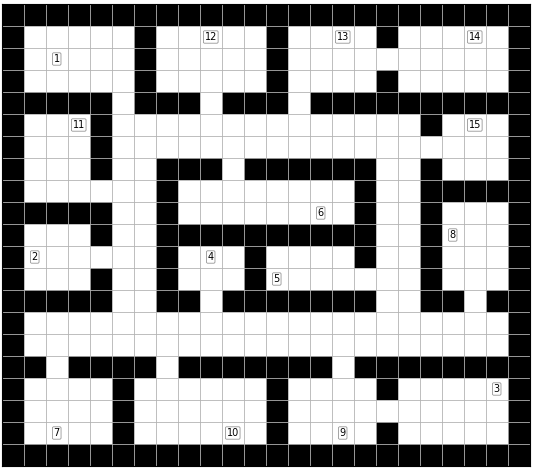
\includegraphics[width=0.80\columnwidth]{../contents/figure/maze.png}
  \caption{迷路環境と各タスクのゴール位置}
  \label{fig:maze}
\end{figure}


\subsection{評価方法}
各trial（episode）$k$で得られる割引累積報酬を 
$W_k$ とし，trial $t$ までの累積平均利得
\begin{equation}
\bar{W}_t=\frac{1}{t}\sum_{k=1}^{t} W_k
\end{equation}
を学習曲線として用いる．実験はソース側で学習した方策を
 $\mathcal{L}$ に格納した後，
ターゲットで各エピソード開始時に方策選択手法により 
$\mathcal{L}\cup\{\pi_{\mathrm{new}}\}$ 
から方策を選択して実行し，
エピソード終了後に推定価値の更新とQ学習による
 $\pi_{\mathrm{new}}$ の更新を繰り返す．
上記を報酬設計1/2の2条件で実施し，3手法の結果を比較する．


% 5章：結果
\section{結果}\label{sec:results}
本章では，報酬設計1（ゴール到達報酬のみ）および
報酬設計2（ステップ負報酬＋壁衝突ペナルティ）における
学習曲線の比較結果を示す．図中のエラーバーは
複数試行（runs=5）におけるばらつきを表す．
以降のPRQにおける方策選択（バンディット）手法は，
事前のグリッドサーチにより各条件で良好であったパラメータを用いた．
具体的には，報酬設計1では 
Boltzmann（$\tau_0=0.0,\, d\tau=0.05$），
$\varepsilon$-greedy（$\varepsilon_b=0.05$），
UCB（$c=0.3$），
報酬設計2では Boltzmann（$\tau_0=0.05,\, d\tau=0.05$），
$\varepsilon$-greedy（$\varepsilon_b=0.2$），
UCB（$c=0.1$）を用いた．
なお，Baseline は$\varepsilon$-greedy による
通常のQ学習である．

\subsection{報酬設計1（ゴール到達報酬のみ）の結果}
報酬設計1においては，いずれのタスクにおいても 
PRQ（方策再利用）系列が Baseline を一貫して上回り，
学習初期から累積平均利得（cumulative mean gain）
がより大きくなる傾向が確認できる．
例えば Task 1（goal=(2,2)）では，3手法はいずれも
 Baseline より高い利得を示し，
 特にUCBが終盤までわずかに高い値を維持した．
 一方で Boltzmann と$\varepsilon$-greedy は
 近い性能で推移し，差は小さい（図1相当）．

Task 5（goal=(12,12)）では，$\varepsilon$-greedy が
学習初期から立ち上がりが速く，終盤まで高い利得を示した．
ただし，$\varepsilon$-greedy はエラーバーが比較的大きく，
試行間のばらつきが大きいことも確認できる．UCBは他2手法より
やや低い曲線となった（図2相当）．

Task 12（goal=(9,1)）および Task 15（goal=(21,5)）では，
UCBとBoltzmannが高い性能を示し，$\varepsilon$-greedy は
それらに比べて明確に低い利得で推移した．特にTask 15では，
UCBが学習初期から大きく優位であり，Boltzmannがそれに続き，
$\varepsilon$-greedy は中盤以降に改善するものの差が残った
（図3，図4相当）．
以上より，報酬設計1では PRQ により Baseline を大きく上回る改善が
得られ，その中でもタスクによって最も有効な方策選択手法が
変化することが示唆される
（例：Task 5では$\varepsilon$-greedyが優位，
Task 12/15ではUCBやBoltzmannが優位）．

\subsection{報酬設計2（ステップ負報酬＋壁衝突ペナルティ）の結果}
報酬設計2では，ステップ負報酬および壁衝突ペナルティの導入により，
累積平均利得が全体として負の領域から推移するタスクが多く見られた．
しかしその場合でも，PRQ系列は Baseline より一貫して
高い値（より負が小さい，あるいは0に近い）を示し，
報酬設計を変更しても方策再利用が学習効率改善に寄与することが
確認できる．

Task 1（goal=(2,2)）では，3手法の曲線はほぼ重なって推移し，
方策選択手法間の差は小さい一方，PRQ系列は 
Baseline を大きく上回った（図5相当）．
Task 5（goal=(12,12)）では，Boltzmannが最も高い利得を示し，
$\varepsilon$-greedy がそれに続いた．
UCBは他2手法より低い曲線となり，
特に終盤で差が残った．

Task 9（goal=(15,19)）および Task 12（goal=(9,1)）では，
UCBが全体として最も高い利得を示し，Boltzmannがそれに続き，
$\varepsilon$-greedy が相対的に低い傾向となった（図7，図8相当）．
このように報酬設計2では，報酬のスケールや負報酬の影響により
曲線の絶対値は変化するものの，PRQ系列の優位性自体は維持され，
さらにタスクによってはUCBが安定して高い性能を示す一方，
Task 5のようにBoltzmannが優位となるケースも確認された．

% --- ここから図（4枚） ---
\begin{figure}[!b]
  \centering
  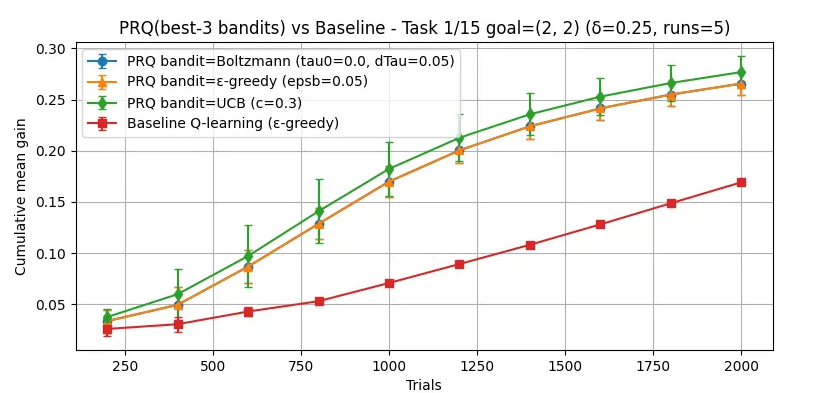
\includegraphics[width=0.90\columnwidth]{../contents/figure/reward1_task01.png}
  \caption{報酬設計1における学習曲線（Task 1）}
  \label{fig:r1_task1}
\end{figure}

\vspace{-1.0em}
\begin{figure}[!b]
  \centering
  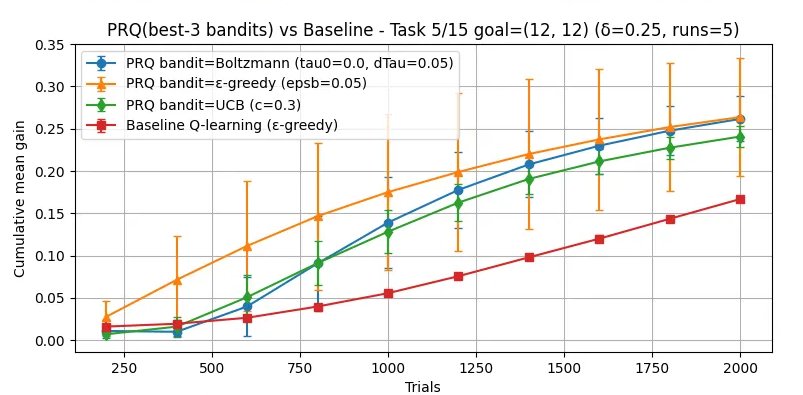
\includegraphics[width=0.90\columnwidth]{../contents/figure/reward1_task05.png}
  \caption{報酬設計1における学習曲線（Task 5）}
  \label{fig:r1_task5}
\end{figure}

\vspace{-1.0em}
\begin{figure}[!b]
  \centering
  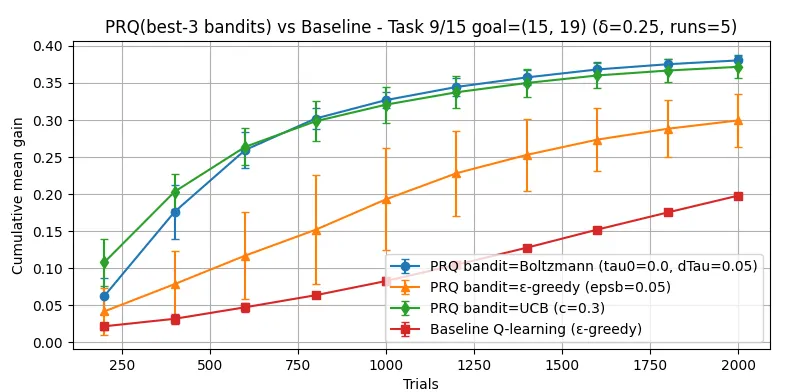
\includegraphics[width=0.90\columnwidth]{../contents/figure/reward1_task09.png}
  \caption{報酬設計1における学習曲線（Task 9）}
  \label{fig:r1_task9}
\end{figure}

\vspace{-1.0em}
\begin{figure}[!b]
  \centering
  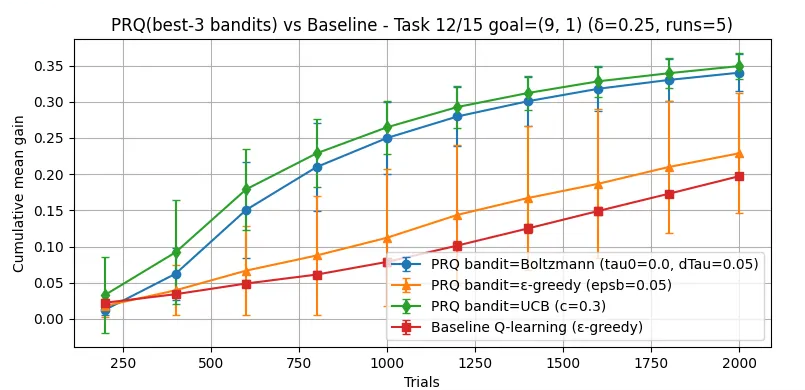
\includegraphics[width=0.90\columnwidth]{../contents/figure/reward1_task12.png}
  \caption{報酬設計1における学習曲線（Task 12）}
  \label{fig:r1_task12}
\end{figure}

%-----ここから６枚

% （前提）プリアンブルに入れておく：
% \usepackage{float}

% 次ページ（次スライド）頭から開始
\clearpage

% --- 残り6枚：左上から縦に並べる（固定配置） ---

\begin{figure}[H]
  \centering
  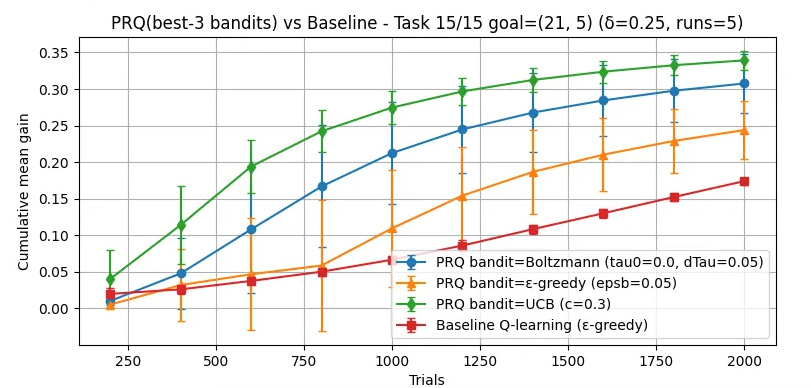
\includegraphics[width=0.90\columnwidth]{../contents/figure/reward1_task15.png}
  \caption{報酬設計1：Task 15}
  \label{fig:r1_task15}
\end{figure}

\vspace{-0.8em}
\begin{figure}[H]
  \centering
  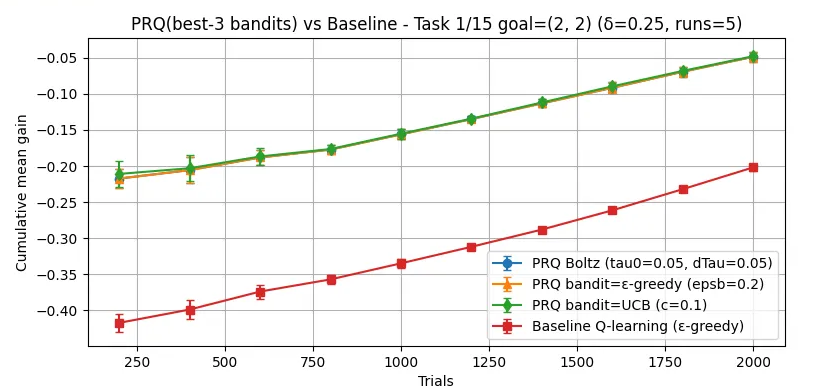
\includegraphics[width=0.90\columnwidth]{../contents/figure/reward2_task01.png}
  \caption{報酬設計2：Task 1}
  \label{fig:r2_task1}
\end{figure}

\vspace{-0.8em}
\begin{figure}[H]
  \centering
  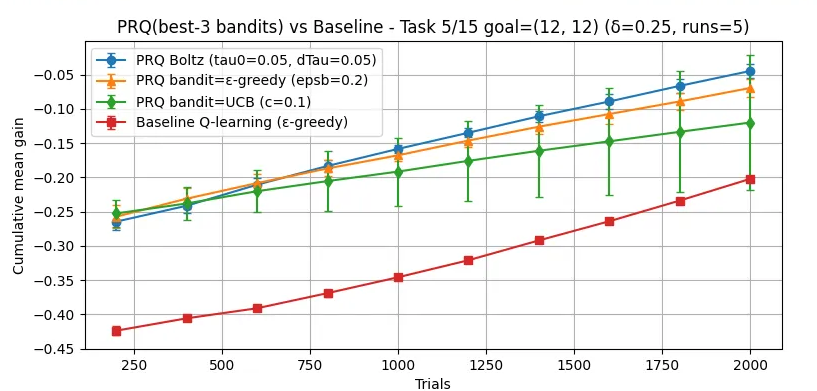
\includegraphics[width=0.90\columnwidth]{../contents/figure/reward2_task05.png}
  \caption{報酬設計2：Task 5}
  \label{fig:r2_task5}
\end{figure}

\vspace{-0.8em}
\begin{figure}[H]
  \centering
  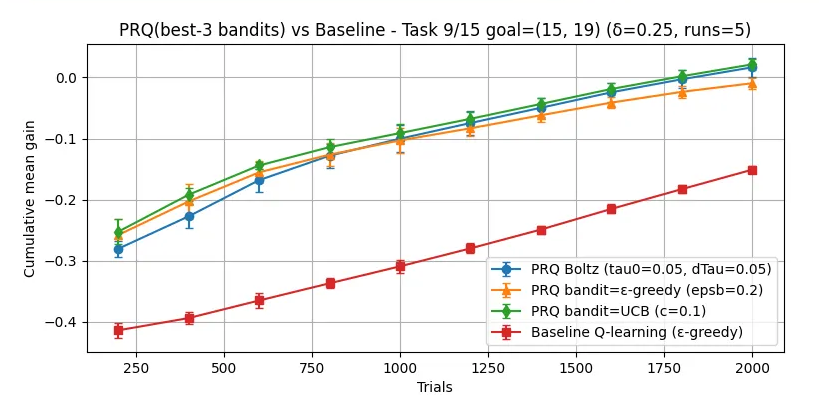
\includegraphics[width=0.90\columnwidth]{../contents/figure/reward2_task09.png}
  \caption{報酬設計2：Task 9}
  \label{fig:r2_task9}
\end{figure}

\vspace{-0.8em}
\begin{figure}[H]
  \centering
  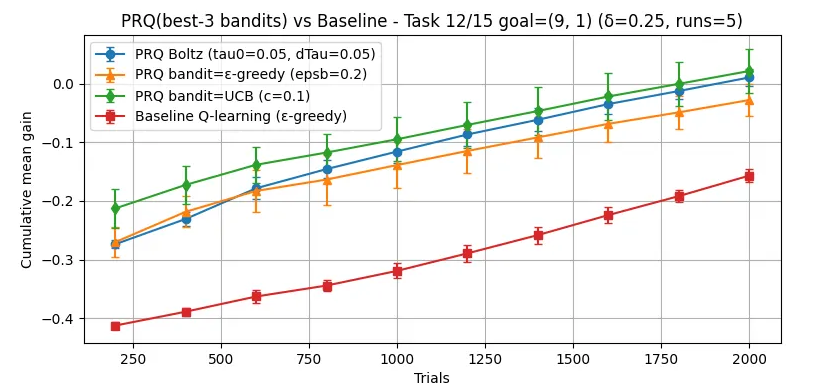
\includegraphics[width=0.90\columnwidth]{../contents/figure/reward2_task12.png}
  \caption{報酬設計2：Task 12}
  \label{fig:r2_task12}
\end{figure}

\vspace{-0.8em}
\begin{figure}[H]
  \centering
  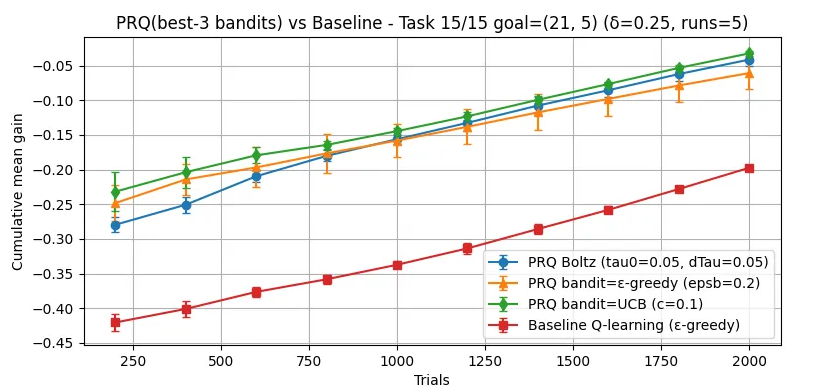
\includegraphics[width=0.90\columnwidth]{../contents/figure/reward2_task15.png}
  \caption{報酬設計2：Task 15}
  \label{fig:r2_task15}
\end{figure}


% 6章：考察
\section{考察}
本章では，結果章で得られた学習曲線の傾向について，
(i) 方策選択（バンディット）手法の特性，
(ii) 報酬設計の変更による影響
の観点から考察する．

\subsection{方策選択手法による性能差}
報酬設計1において，PRQ系列はいずれのタスクでもBaselineを上回り，
方策再利用が学習初期の性能向上に寄与することが確認できた．
一方で，PRQ内の方策選択手法
（Boltzmann，$\varepsilon$-greedy，UCB）の優劣は
タスクに依存して変化した．
Task 5では$\varepsilon$-greedyが立ち上がりが速く高い性能を示したが，
エラーバーが比較的大きく，
試行間のばらつきが大きい傾向も見られた．
$\varepsilon$-greedyは探索が一様であるため，
偶然有効な方策を早期に引き当てた場合には急速に性能が伸びる一方，
引き当てのタイミングが遅れる試行では学習が遅れ，
分散が大きくなりやすいと解釈できる．

一方，Task 12やTask 15ではUCBおよびBoltzmannが優位であり，
$\varepsilon$-greedyは相対的に低い性能に留まった．
UCBは推定価値に不確実性（選択回数の少なさ）を加点することで，
未探索の方策を段階的に試す方向へ選択を誘導する．
そのため，タスクによって有効な方策が変化しやすい条件や，
初期の推定値が不安定な条件では，
$\varepsilon$-greedyよりも探索が安定し，
高い性能に繋がった可能性がある．
Boltzmannも確率的に複数方策を試しながら価値差に応じて
選択確率を変化させるため，
UCBほどの探索保証はないものの，
温度の設定次第で探索と活用のバランスを滑らかに調整でき，
タスクによってはUCBに近い挙動を示したと考えられる．

\subsection{報酬設計の変更による影響}
報酬設計2では，ステップ負報酬および壁衝突ペナルティを導入したため，
累積平均利得が負の領域から推移するタスクが多く見られた．
この変化は「ゴール到達だけでなく，
途中の行動コストを明示的に最適化対象へ含めた」ことに対応している．
しかし，利得の絶対値が変化しても，
PRQ系列がBaselineを一貫して上回る傾向は維持されており，
方策再利用の効果は報酬構造の変更に対して比較的頑健であることが
示唆される．

一方で，PRQ内の3手法の関係は報酬設計によって変化した．
例えばTask 5では報酬設計2でBoltzmannが最も高い利得を示し，
UCBが相対的に低くなった．
これは，負報酬を導入したことで短期的なコストの違いが価値推定に
反映されやすくなり，価値差に応じて確率的に選択を集中させる
Boltzmannが有利に働いた可能性がある．
一方，Task 9やTask 12ではUCBが高い性能を維持しており，
ペナルティ導入により探索が難しくなった状況でも，
不確実性を考慮した選択が有効なケースが存在することが分かる．
このことから，報酬設計は「どの方策選択が有利か」
を変えうる要因であり，単一条件で得た結論を一般化するには
注意が必要である．

\subsection{限界と今後の課題}
本研究の比較は，迷路環境および設定した2種類の報酬設計に基づくものであり，
報酬スケールや迷路構造，方策ライブラリの多様性が変化した場合に
同様の傾向が再現されるかは追加検証が必要である．
また，本研究ではグリッドサーチによりパラメータを選定したが，
実運用を想定するとタスクごとに広範な探索を行うことはコストが高い．
今後は，環境の特徴量や学習進行に応じてパラメータを自動調整する手法
（適応的温度制御や探索率制御）を導入し，
チューニング負荷を低減することが課題となる．
さらに，関数近似を用いる大規模状態空間や深層強化学習への拡張，
複数のソース環境からの方策選択なども検討対象となる．


% 7章：おわりに
\section{おわりに}
本研究では，環境変化に対して迅速に適応する強化学習の実現に向け，
方策再利用（Policy Reuse）の枠組みにおける方策選択に着目し，
既存研究で用いられているボルツマン選択に加えて 
$\varepsilon$-greedy および UCB を導入した比較実験を行った．
さらに，報酬設計を2種類（ゴール到達報酬のみ，
およびステップ負報酬＋壁衝突ペナルティ）用意し，
報酬構造の変更が各方策選択手法の挙動と性能差に与える影響も検証した．
その結果，いずれの報酬設計においても
方策再利用を用いるPRQ系列はBaseline（通常のQ学習）を
一貫して上回り，転移（再利用）による学習効率向上が確認できた．
一方で，PRQ内の方策選択手法の優劣はタスクや報酬設計に依存して
変化し，単一の手法が常に最良となるわけではないことが示唆された．

今後の課題として，
より多様な迷路構造や報酬スケールに対する再現性検証に加え，
グリッドサーチに依存しない形で探索パラメータを自動調整する手法の
導入が挙げられる．
また，本研究は表形式のQ学習を前提としたが，
より大規模な状態空間や実問題への適用を想定すると，
関数近似や深層強化学習への拡張が重要となる．
加えて，複数のソース環境から得られた方策を
ライブラリに蓄積する状況では，
方策の選択・管理戦略そのものが性能に直結するため，
方策集合の構成方法や選択基準の高度化も検討すべきである．
これらの検討を通じて，環境変化を伴う実運用場面においても
頑健かつ効率的に学習できる転移強化学習手法の確立を目指す．


\vspace{2em}
% 謝辞
\input{deim-acknowledgment}


%\vspace{30mm} <- 文献が本文と近すぎるときは適宜利用してください．
\vspace{2em}

\begin{thebibliography}{99}

\bibitem[1]{Fernandez2006}
F. Fern{\'a}ndez and M. Veloso,
``Probabilistic Policy Reuse in a Reinforcement Learning Agent,''
in \textit{Proc. of the 5th Int. Joint Conf. on Autonomous Agents and Multiagent Systems (AAMAS)},
pp.~720--727, 2006.

\bibitem[2]{SuttonBarto1998}
R. S. Sutton and A. G. Barto,
\textit{Reinforcement Learning: An Introduction},
MIT Press, 1998.

\bibitem[3]{WatkinsDayan1992}
C. J. C. H. Watkins and P. Dayan,
``Q-learning,''
\textit{Machine Learning},
Vol.~8, No.~3--4, pp.~279--292, 1992.

\bibitem[4]{Thrun1995}
S. Thrun,
``Is Learning the N-th Thing Any Easier than Learning the First?,''
in \textit{Advances in Neural Information Processing Systems (NIPS)},
pp.~640--646, 1995.

\bibitem[5]{TaylorWhitesonStone2007}
M. E. Taylor, S. Whiteson, and P. Stone,
``Transfer via Inter-task Mappings in Policy Search Reinforcement Learning,''
in \textit{Proc. of the Int. Conf. on Autonomous Agents and Multiagent Systems (AAMAS)},
pp.~37--44, 2007.

\bibitem[6]{TaylorKuhlmannStone2008}
M. E. Taylor, G. Kuhlmann, and P. Stone,
``Autonomous Transfer for Reinforcement Learning,''
in \textit{Proc. of the Int. Conf. on Autonomous Agents and Multiagent Systems (AAMAS)},
pp.~283--290, 2008.

\bibitem[7]{MaclinShavlik1996}
S. Maclin and J. W. Shavlik,
``Creating Advice-Taking Reinforcement Learners,''
\textit{Machine Learning},
Vol.~22, No.~1--3, pp.~251--281, 1996.

\bibitem[8]{NicolescuMataric2003}
M. Nicolescu and M. J. Matari{\'c},
``Natural Methods for Robot Task Learning: Instructive Demonstrations, Generalization and Practice,''
in \textit{Proc. of the Int. Conf. on Autonomous Agents and Multiagent Systems (AAMAS)},
pp.~241--248, 2003.

\bibitem[9]{BartoMahadevan2003}
A. G. Barto and S. Mahadevan,
``Recent Advances in Hierarchical Reinforcement Learning,''
\textit{Discrete Event Dynamic Systems},
Vol.~13, No.~4, pp.~341--379, 2003.

\bibitem[10]{KonidarisBarto2007}
G. Konidaris and A. G. Barto,
``Building Portable Options: Skill Transfer in Reinforcement Learning,''
in \textit{Proc. of the 20th Int. Joint Conf. on Artificial Intelligence (IJCAI)},
pp.~895--900, 2007.

\bibitem[11]{Auer2002}
P. Auer, N. Cesa-Bianchi, and P. Fischer,
``Finite-time Analysis of the Multiarmed Bandit Problem,''
\textit{Machine Learning},
Vol.~47, No.~2--3, pp.~235--256, 2002.

\end{thebibliography}


\end{document}
